\documentclass[a4paper]{scrartcl}

\usepackage[ngerman]{babel}
\usepackage[utf8]{inputenc}   % Umlaute etc. verwenden
\usepackage[final]{graphicx}    % Grafiken einbinden
\usepackage{url}
\usepackage{float}
\usepackage{framed}
\usepackage{wrapfig}
\parindent 0pt
\usepackage[onehalfspacing]{setspace}

% direkt PDF generieren
\usepackage[pdftex,
    pdftitle={SiLift - Benutzerhandbuch für Endanwender},
	pdfauthor={}]{hyperref}
    
% Bis zu welcher Tiefe nummerieren?
\setcounter{secnumdepth}{3}


\begin{document}

% Der Titel der Seminararbeit, sowie der Autor
\title{SiLift - Benutzerhandbuch für Endanwender}
%\author{}

%\date{\today}

\maketitle

%*************************************************************************
%\section{Abstract}
%*************************************************************************
%\begin{abstract}

%\end{abstract}

\newpage

%INHALTSVERZEICHNIS
\tableofcontents
\newpage

%*************************************************************************
\section{Einleitung}
%*************************************************************************

\textit{SiLift} ist ein \textit{Eclipse-}basiertes Framework mit dessen Hilfe sich Differenzen von \textit{EMF-Modellen} \textit{semantisch liften} lassen.
Des Weiteren kann SiLift dazu verwendet werden auf Basis einer solchen Differenz einen \textit{Patch} zu generieren, um diesen auf ein anderes Modell anzuwenden.
Ebenfalls besteht die Möglichkeit des \textit{3-Wege-Mischens} mit entsprechender Konflikterkennung.\\
Dieses Benutzerhandbuch umfasst eine Installationsanleitung sowie einführende Tutorials zur Anwendung von SiLift als Endanwender.
%*************************************************************************
\section{Voraussetzung und Installation}
%*************************************************************************

SiLift ist als \textit{Eclipse-Feature} unter folgender \textit{Update-Site} erhältlich:\\ \url{http://pi.informatik.uni-siegen.de/Projekte/SiLift/updatesite}.\\

\textbf{Hinweis:} Vergewissern Sie sich, ob ihr Eclipse die notwendigen Voraussetzungen erfüllt. 
Eine Liste der benötigten Plugins ist unter \url{http://pi.informatik.uni-siegen.de/Projekte/SiLift/download.php} zu finden.
Bitte beachten Sie dabei die entsprechenden Hinweise zu den jeweiligen Versionen.\\

Sofern alle Voraussetzungen erfüllt sind, kann SiLift wie gewohnt über den Menüpunkt \texttt{Help} $\triangleright$ \texttt{Install New Software...} installiert werden (Abb. \ref{eclipse_install_new_software}).
\begin{figure}[H]
\centering
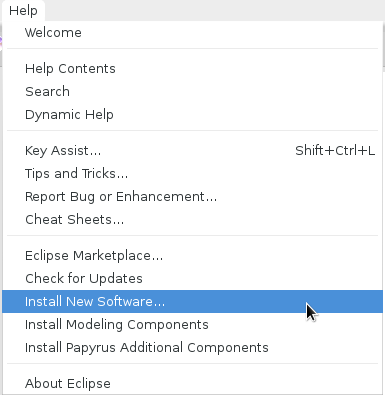
\includegraphics[width=0.25\textwidth]{graphics/eclipse-install_new_software.png}
\caption{Eclipse: Install New Software...}
\label{eclipse_install_new_software}
\end{figure}

Es sollten Ihnen vier Kategorien angezeigt werden (vgl. Abb. \ref{silift_update_site}). 

\begin{figure}[H]
\centering
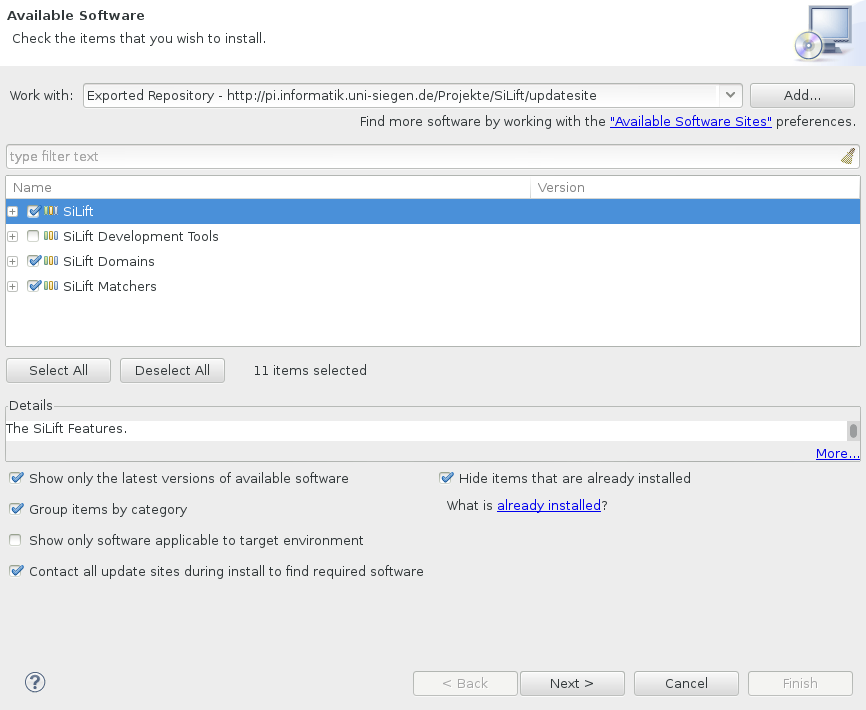
\includegraphics[width=0.5\textwidth]{graphics/eclipse-install_silift.png}
\caption{SiLift Update Site}
\label{silift_update_site}
\end{figure}

Für die folgenden Tutorials benötigen wir alle Features aus der Kategorie \texttt{SiLift},  das Feature \texttt{SiLift Ecore Domain} aus der Kategorie \texttt{SiLift Domains}, sowie den \texttt{SiLift Named Element} und \texttt{SiLift UUID Matcher} aus \texttt{SiLift Matchers}. Sie könnenn aber auch wie in Abbildung \ref{silift_update_site} die kompletten Kategorien auswählen. Danach klicken Sie auf \texttt{Next} und folgen dem Installationsassistenten.\\

\textbf{Hinweis}: Generell unterstützt SiLift alle \textit{EMF-basierten} Modellierungsprachen, sofern die ent\-sprech\-enden \textit{Editieroperationen} implementiert wurden.
In der aktuellen Version stehen diese bereits für \textit{Ecore-} und \textit{Feature-Modelle} zur Verfügung.\footnote{Informationen zur Integration weiterer Modelltypen finden Sie im \textbf{SiLift - Benutzerhandbuch für Entwickler}.}\\

%*************************************************************************
\section{SiLift benutzen}
%*************************************************************************
%************************
\subsection{Vergleich von Modellen}
%************************
Die Bedienung von SiLift als Vergleichswerkzeug soll am folgenden Beispiel demonstriert werden.
Ausgangsbasis sind die \textit{Ecore-Modelle} in Abbildung \ref{classdiagram_example}.

\begin{figure}[H]
\centering
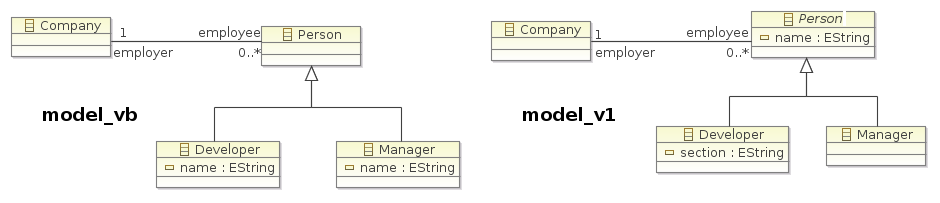
\includegraphics[width=\textwidth]{graphics/ecore-classdiagram_example.png}
\caption{Ecore-Modelle}
\label{classdiagram_example}
\end{figure}

Dabei stellt \texttt{model\_vb} das Ausgangsmodell und \texttt{model\_v1} das im Laufe eines Entwicklungsprozesses veränderte Modell dar.
Die entscheidenden Änderungen sind zum einen das Attribut \texttt{name}, welches durch den Entwicklungsprozess in die nun \textit{abstrakte} Klasse \texttt{Person} verschoben wurde und das neue Attribut \texttt{section} in der Klasse \texttt{Developer}.\\
Als nächstes selektieren Sie die beiden \textit{ecore}-Files im \textit{Package Explorer} und öffnen mit der rechten Maustaste das Kontextmenü.
Wählen Sie \texttt{SiLift} $\triangleright$ \texttt{Compare with each other} aus (vgl. Abb. \ref{silift-contextmenu_compare}).

\begin{figure}[H]
\centering
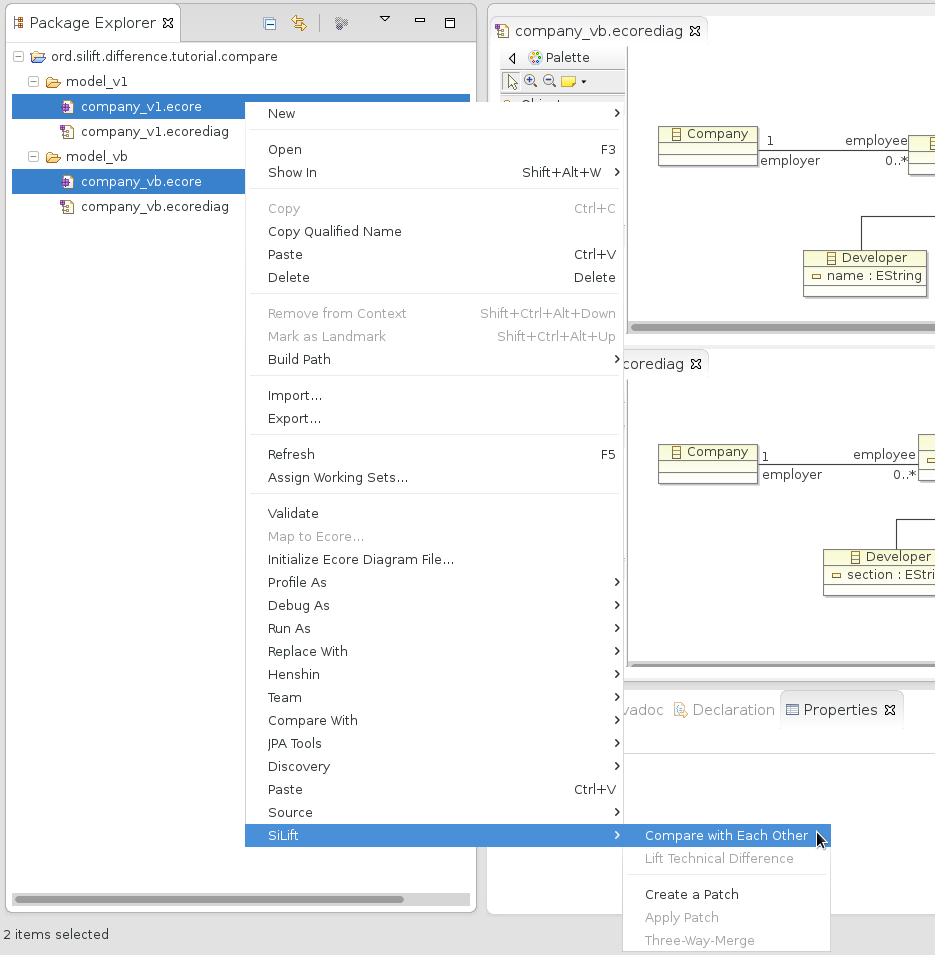
\includegraphics[width=0.7\textwidth]{graphics/silift-contextmenu_compare.png}
\caption{SiLift über das Kontextmenü starten}
\label{silift-contextmenu_compare}
\end{figure}

Es öffnet sich ein Wizard-Dialog, der sich über zwei Seiten erstreckt und mehrere Konfigurationsmöglichkeiten bietet (Abb. \ref{silift-wizard_compare_page1} und \ref{silift-wizard_compare_page2}).
Um diese besser zu verstehen, folgt ein kleiner Exkurs über die Architektur von \textit{SiLift}.

\begin{figure}[H]
\centering
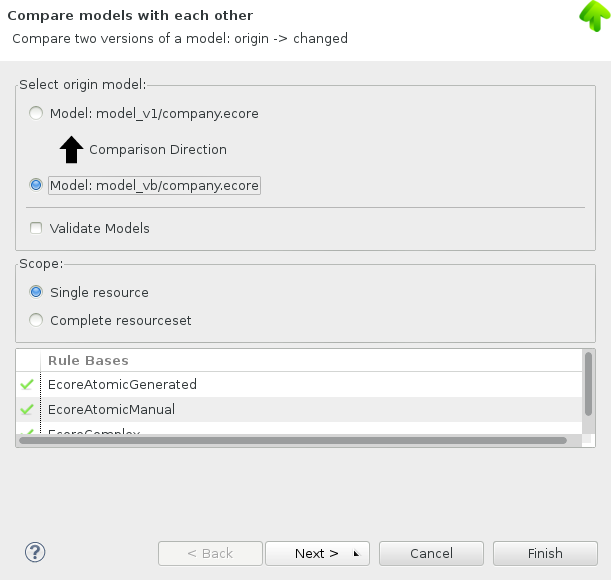
\includegraphics[width=0.5\textwidth]{graphics/silift-wizard_compare_page1.png}
\caption{Einstellungen für das Erstellen gelifteter Differenzen: Seite 1}
\label{silift-wizard_compare_page1}
\end{figure}

\begin{figure}[H]
\centering
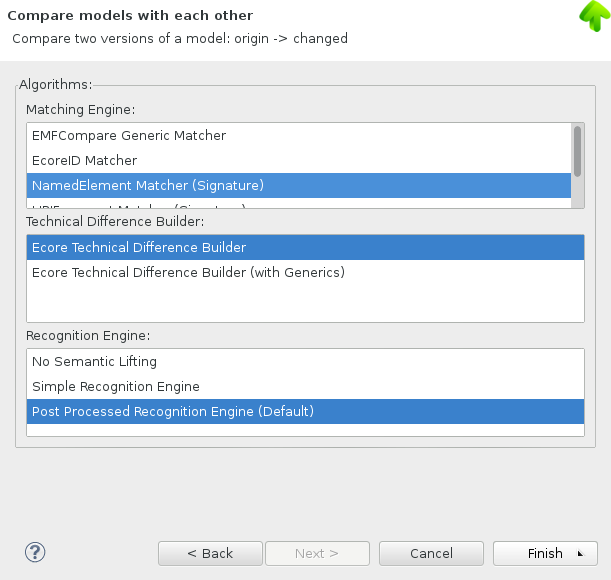
\includegraphics[width=0.5\textwidth]{graphics/silift-wizard_compare_page2.png}
\caption{Einstellungen für das Erstellen gelifteter Differenzen: Seite 2}
\label{silift-wizard_compare_page2}
\end{figure}

\subsubsection*{Exkurs: Differenz-Pipeline}

\begin{figure}[H]
\centering
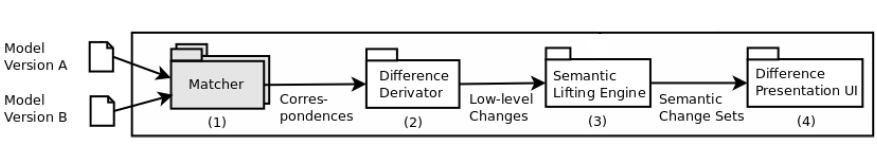
\includegraphics[width=\textwidth]{graphics/eclipse-SiLift_pipeline.png}
\caption{SiLift Processing Pipeline}
\label{install_SiLift_pipeline}
\end{figure}

Die Vorgehensweise von SiLift lässt sich am besten mit einer vierstufigen \textit{Pipeline}, wie in Abbildung \ref{install_SiLift_pipeline} dargestellt,  vergleichen.
Als Eingabe dienen immer zwei Versionen eines Modells, z.B. \texttt{model\_A.ecore} und \texttt{model\_B.ecore} (Abb. \ref{classdiagram_example}):

\begin{enumerate}
\item \textbf{Matching}: Aufgabe eines \textit{Matcher} ist es die korrespondierenden Elemente aus Modell A und Modell B, also die Elemente, die in beiden Modellen übereinstimmen, zu identifizieren.
Dabei ist das Ergebnis vor allem davon abhängig anhand welcher Kriterien der Matcher eine Übereinstimmung festlegt.
Hier wird unter anderem unterschieden zwischen \textit{ID-}, \textit{signatur-} und \textit{ähnlichkeitsbasierten} Verfahren.\\
In SiLift stehen unter anderem folgende Matcher-Engines zur Verfügung:

\begin{itemize}
	\item \texttt{EcoreID Matcher}:
	\item \texttt{EMF Compare}: Unterstützt alle drei Verfahren. \texttt{EMF Compare} kann unter \texttt{Win\-dow} $\triangleright$ \texttt{Preferences}: \texttt{EMF Compare} konfiguriert werden. \footnote{Informationen zum \texttt{EMF Compare Project} finden Sie unter \url{http://www.eclipse.org/emf/compare}.}
	
	\item \texttt{NamedElement Matcher}: Ein signaturbasierter Matcher, welcher die ent\-sprech\-enden Korrespondenzen anhand der Werte der jeweiligen Namensattribute bestimmt.
	
	\item \texttt{URIFragment Matcher}: Ein signaturbasierter Matcher, welcher die ent\-sprech\-enden Korrespondenzen anhand der Werte der \textit{Uri} der Elemente bestimmt (z.B. \texttt{eType=}"'\texttt{ecore:EDataType http://www.eclipse.org/emf/2002/\-E\-core\-\#//EString}"').
	
	\item \texttt{UUID Matcher}: Ein ID-basierter Matcher.
\end{itemize}
(Abb. \ref{silift-wizard_compare_page2}).
Diese Liste ist keineswegs abgeschlossen und kann durch zusätzliche Matching-Engines, wie z.B. \textit{SiDiff} oder auch eigener Matcher ergänzt werden.\footnote{Weitere Informationen zu \textit{SiDiff} finden Sie unter \url{http://pi.informatik.uni-siegen.de/Projekte/sidiff}}\\

\item \textbf{Difference derivation}: Ausgehend von den gefunden Korrespondenzen berechnet der \textit{Difference Derivator} eine technische Differenz (\textit{low-level difference}) der Mo\-del\-le.
Alle Objekte und Referenzen, für die keine Korrespondenz existiert müssen demnach entweder in Modell B hinzugefügt, oder aus Modell A entfernt worden sein (vgl. Abb. \ref{silift-technical_difference}).

\begin{figure}[H]
\centering
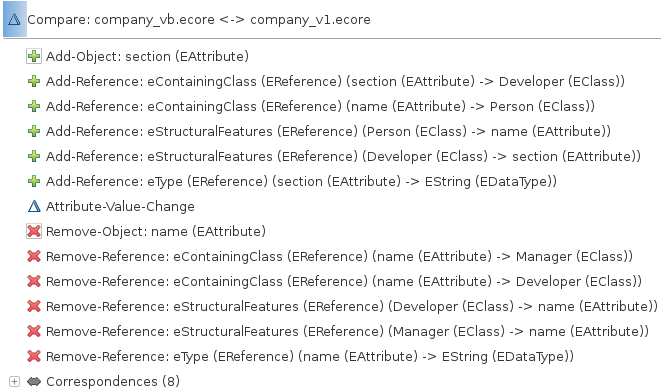
\includegraphics[width=0.8\textwidth]{graphics/silift-technical_difference.png}
\caption{technische Differenz von  \texttt{model\_vb.ecore} und \texttt{model\_v1.ecore}}
\label{silift-technical_difference}
\end{figure}

Die Berechnung der technischen Differen kann durch die Wahl des \textit{Technical Difference Builder} beeinflusst werden (vgl. Abb. \ref{silift-wizard_compare_page2}).

\item \textbf{Semantic Lifting}: Die zuvor berechnete technische Differenz enthält alle Änder\-ungen auf Basis des Metamodells.
Diese sollen nun \textit{semantisch geliftet} werden.
Dazu werden die einzelnen Änderungen mit Hilfe von \textit{Erkennungsregeln} (egnl. \textit{recognition rules}) in sogenannte \textit{Semantic Change Sets} gruppiert, die jeweils eine vom Benutzer ausgeführte \textit{Editieroperation} repräsentieren.
Mit der Wahl einer \textit{Rule Base} wird festgelegt, welche Erkennungsregeln zum liften benutzt werden sollen.
Dabei wird zwischen folgenden \textit{Rule Bases} unterschieden: \texttt{AtomicGenerated}, \texttt{Atomic\-Manual} und \texttt{Complex} (vgl. Abb. \ref{silift-wizard_compare_page1}).
Während atomare Regeln das Erzeugen, Löschen, Verschieben von Elementen und das Ändern der Attributwerte von Elementen umfassen, setzen sich die komplexen Editierregeln i.d.R. aus den atomaren und anderen komplexen Regeln zusammen.\footnote{Weitere Informationen zu den \textit{Recognition Rules} finden Sie im \textbf{SiLift - Benutzerhandbuch für Entwickler}.}
Welchen Einfluss die Wahl einer oder mehrerer \textit{Rule Bases} für das \textit{semantische Liften} hat wird später noch am Beispiel demonstriert.

\item \textbf{Difference Presentation UI}: \textit{SiLift} stellt zwei Benutzerschnittstellen (egnl. \textit{User Interfaces}) zur Verfügung, um die semantisch gelifteten Differenzen anzuzeigen: einen Baum-basierten (Abb. \ref{eclipse-SiLift_namedElement_atomic}) und einen grafischen Editor (Abb. \ref{eclipse-SiLift_ComapreView_atomic}).
\end{enumerate}

Damit endet die Pipeline.
Über den Wizard kann man an jeder Position der Pipeline eingreifen und somit das Verhalten von SiLift beeinflussen. Zusätzlich lassen sich noch folgende Einstellungen vornehmen:
%Was jetzt noch fehlt, sind die Optionen \textit{Select source model}, \textit{Merge Imports}, \textit{Recognition-Engine} und der \textit{Comparison mode}:
\begin{itemize}

\item \textbf{Select source model}: Die Differenzberechnung zwischen zwei Modellen ist nicht kommutativ.
I.d.R. handelt es sich bei den zu vergleichenden Modellen um unterschiedliche Revisionen ein und desselben Modells.
In den meisten Fällen wird man die älter Revision (Modell VB) mit der neueren (Modell V1) vergleichen wollen.
Dennoch kann auch der andere Fall eintreten.
In \textit{Select source model} können Sie die Richtung der Differenzberechnung festlegen.\\
Zusätzlich kann man die Modelle vor der Differenzbildung noch validieren (vgl. Abb. \ref{silift-wizard_compare_page1}).

%\item \textbf{Merge Imports}: Diese Option ist in der aktuellen Version entfernt worden.
%Modelle können andere Modelle importieren und auf Objekte dieser referenzieren. Ist dies der Fall muss diese Option aktiviert sein, damit auch diese Modelle bzw. die referenzierten Objekte berücksichtigt werden.

\item \textbf{Scope}: Ein Modell muss nicht in sich geschlossen sein, sondern kann auf andere Modelle bzw. deren Elemente verweisen.
Mit Hilfe des Scopes kann man festlegen, ob diese Modelle bei der Erzeugung der Differenz ignoriert (\texttt{Single resource}), oder mit in diese aufgenommen werden sollen (\texttt{Complete resourceset}, vgl. Abb. \ref{silift-wizard_compare_page1}).


\item \textbf{Recognition-Engine}: Mit der Wahl einer \textit{Recognition-Engine} wird festgelegt, ob und wie die technischen Differenzen geliftet werden.
Wie der Name bereits andeutet, wird bei der Auswahl von \texttt{No Semantic Lifting} keine semantische Differnz erzeugt.
Für das Erzeugen einer semantischen Differenz stehen zum einen die \texttt{Simple Recognition Engine}, zum anderen die \texttt{Post Processed Recognition Engine} zur Verfügung.
Der Unterschied liegt im Auftreten von Überlappungen der \textit{Semantic Change Sets}, die vor allem bei der zusätzlichen Verwendung von komplexen \textit{Rule Bases} auftreten.
Wenn Sie komplexe Erkennungsregeln nutzen (und auch sonst) ist es daher ratsam die \texttt{Post Processed Recognition Engine} zu nutzen, um eben diese Überlappungen zu vermeiden (vgl. Abb. \ref{silift-wizard_compare_page2}).

\end{itemize}

Nachdem Sie nun die Konfigurationsmöglichkeiten kennengelernt haben wird es Zeit \textit{SiLift} auf die zuvor erstellten Modelle anzuwenden.
In unserem Beispiel ist \texttt{company\_vb} unsser Basismodell. Des Weiteren wählen wir den \texttt{NamedElement Matcher} und deaktivieren zunächst die komplexen Erkennungsregeln (vgl. Abb. \ref{silift-tutorial_compare_config}).

\begin{figure}[H]
\centering
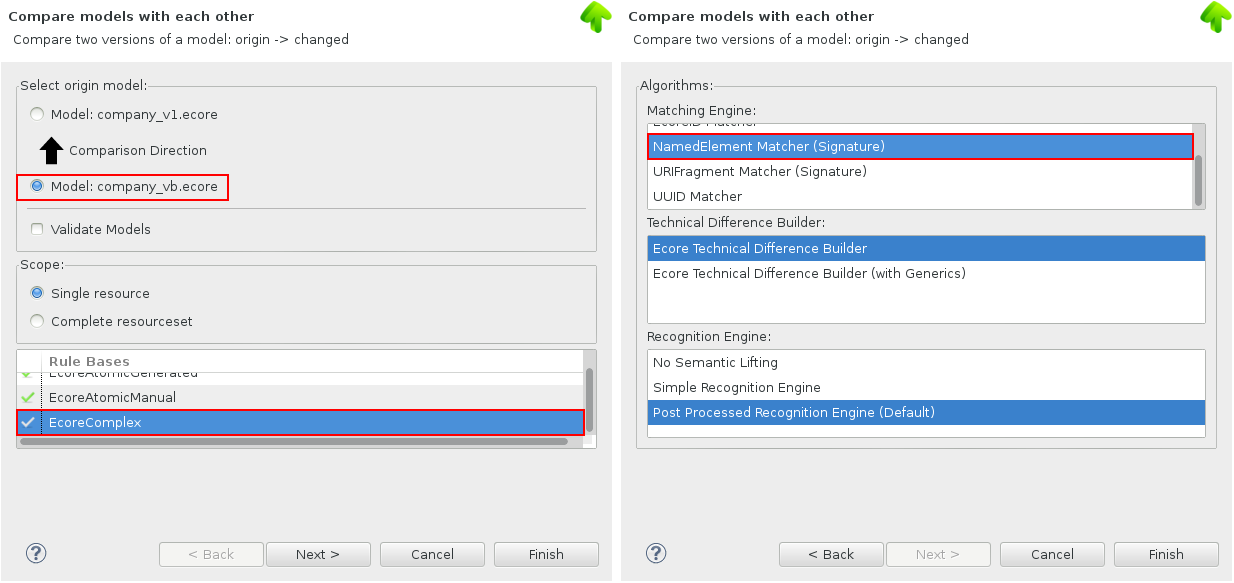
\includegraphics[width=0.8\textwidth]{graphics/silift-tutorial_compare_config.png}
\caption{Einstellungen für das Erstellen einer gelifteten Differenz ohne komplexe Erkennungsregeln}
\label{silift-tutorial_compare_config}
\end{figure}

Das Ergebnis wird in der \texttt{company\_vb\_x\_company\_v1\_NamedElement\_lifted\_post\-pro\-cessed.symmetric} gespeichert und lässt sich mit dem \textit{Difference Model Editor} öffnen (vgl. Abb. \ref{silift-tutorial_compare_atomic_lifted}).

\begin{figure}[H]
\centering
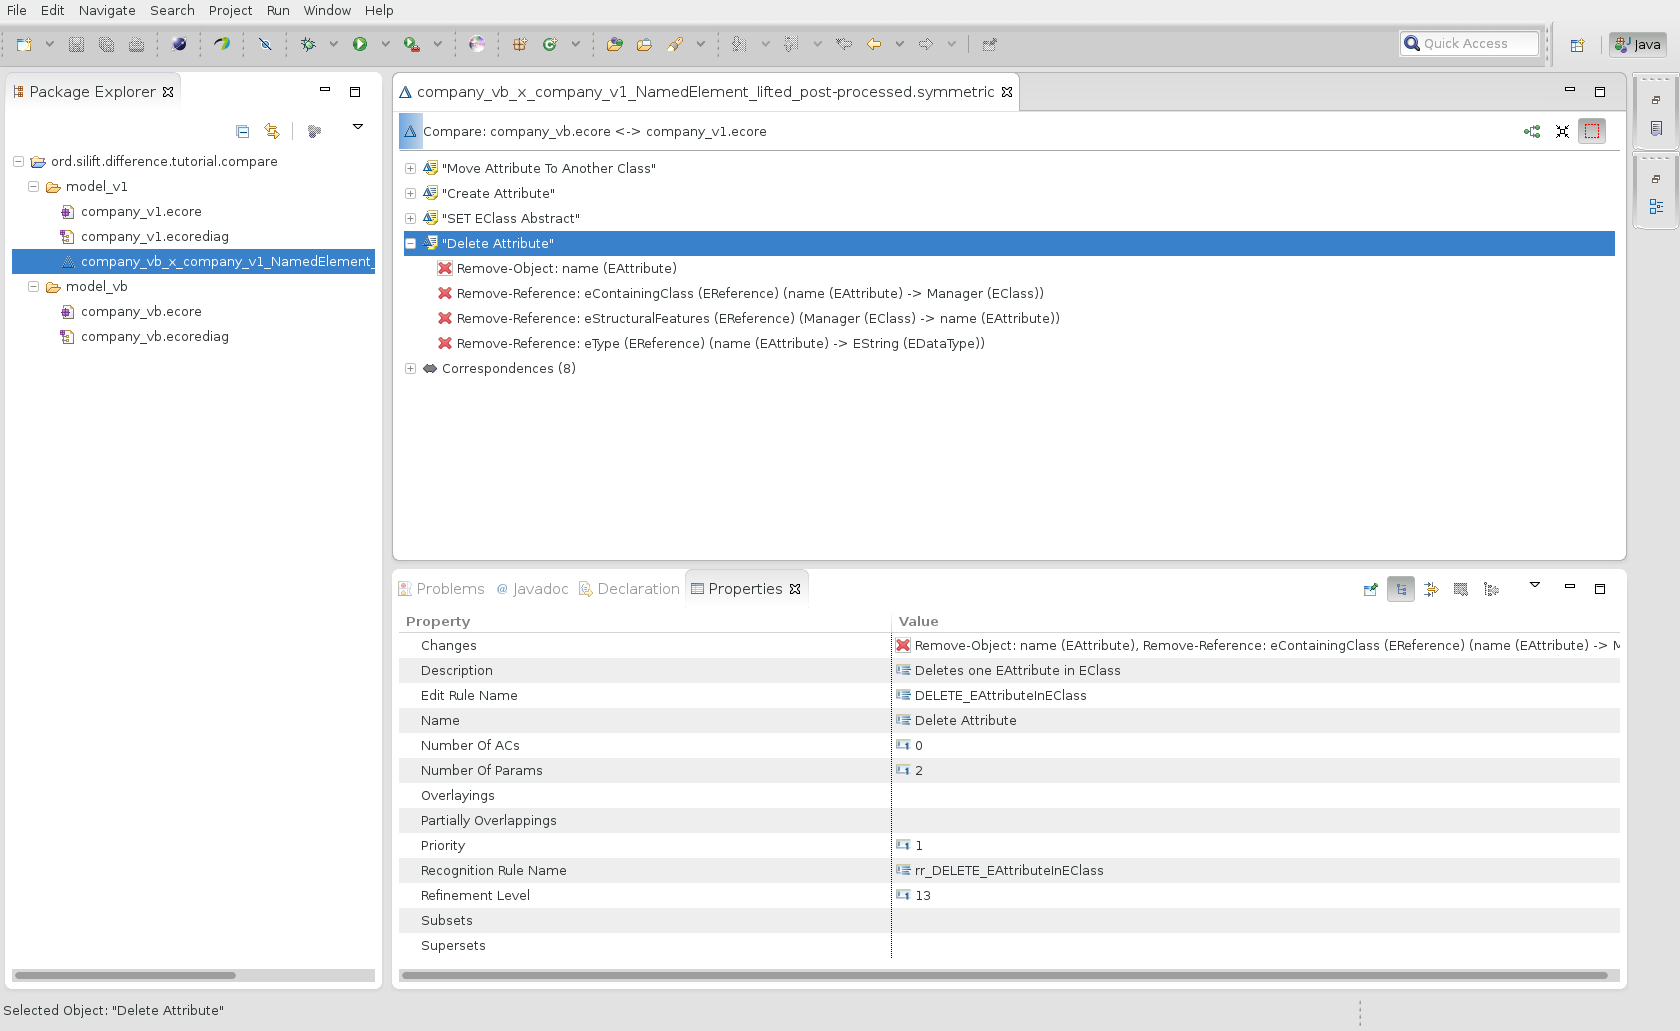
\includegraphics[width=0.8\textwidth]{graphics/silift-tutorial_compare_atomic_lifted.png}
\caption{\texttt{company\_vb\_x\_company\_v1\_NamedElement\_lifted\_post\-pro\-cessed.symmetric}}
\label{silift-tutorial_compare_atomic_lifted}
\end{figure}

Jedes \textit{Sematic Change Set} steht für eine \textit{Editieroperation}, welche im Laufe des Entwicklungszyklus auf Modell VB angewandt wurde.
Somit werden Ihnen die Differenzen nun auf eine intuitive Weise präsentiert, ohne dass Sie das Metamodell in alle Einzelheiten kennen müssen.
Durch das Aufklappen eines Change Sets können jedoch die jeweiligen technischen Differenzen weiterhin angezeigt werden (vgl. Abb. \ref{silift-tutorial_compare_atomic_lifted}).
Zusätzlich werden die gefundenen Korrespondenzen aufgelistet.\\
Neben dem baumbasierten Editor lassen sich die Differenzen mittels eines graphischen Editors anzeigen.
Dieser lässt sich, wie in Abbildung \ref{silift-tutorial_compare_arrange_compare_view} dargestellt, aufrufen.

\begin{figure}[H]
\centering
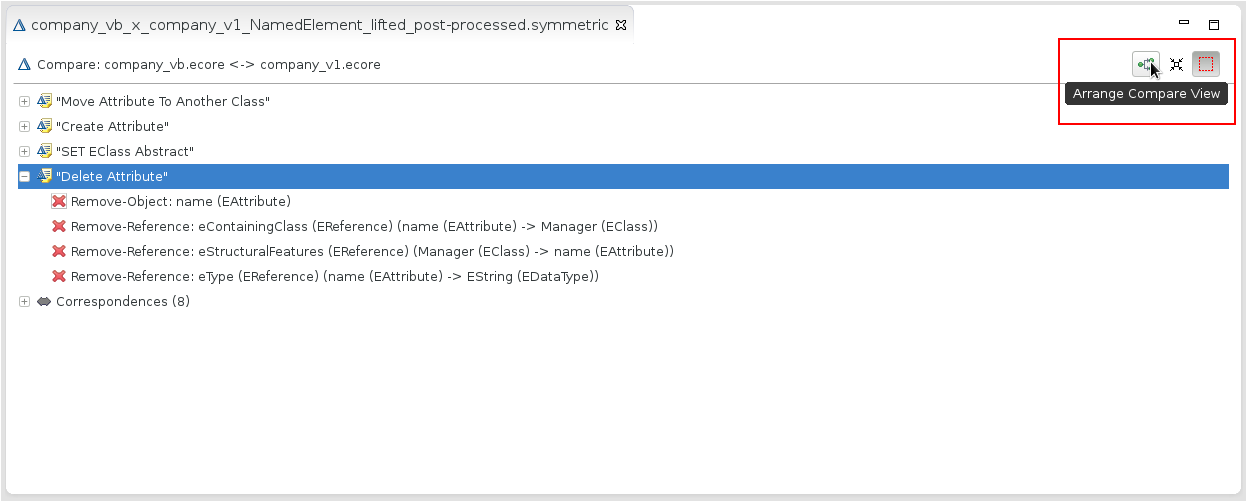
\includegraphics[width=0.6\textwidth]{graphics/silift-tutorial_compare_arrange_compare_view.png}
\caption{Aufruf des graphischen Editors (Compare View)}
\label{silift-tutorial_compare_arrange_compare_view}
\end{figure}

Durch Auswahl eines Change Sets werden die betroffenen Elemente in den Diagrammen \textit{gehighlightet} (vgl. Abb. \ref{silift-tutorial_compare_compare_view}).

\begin{figure}[H]
\centering
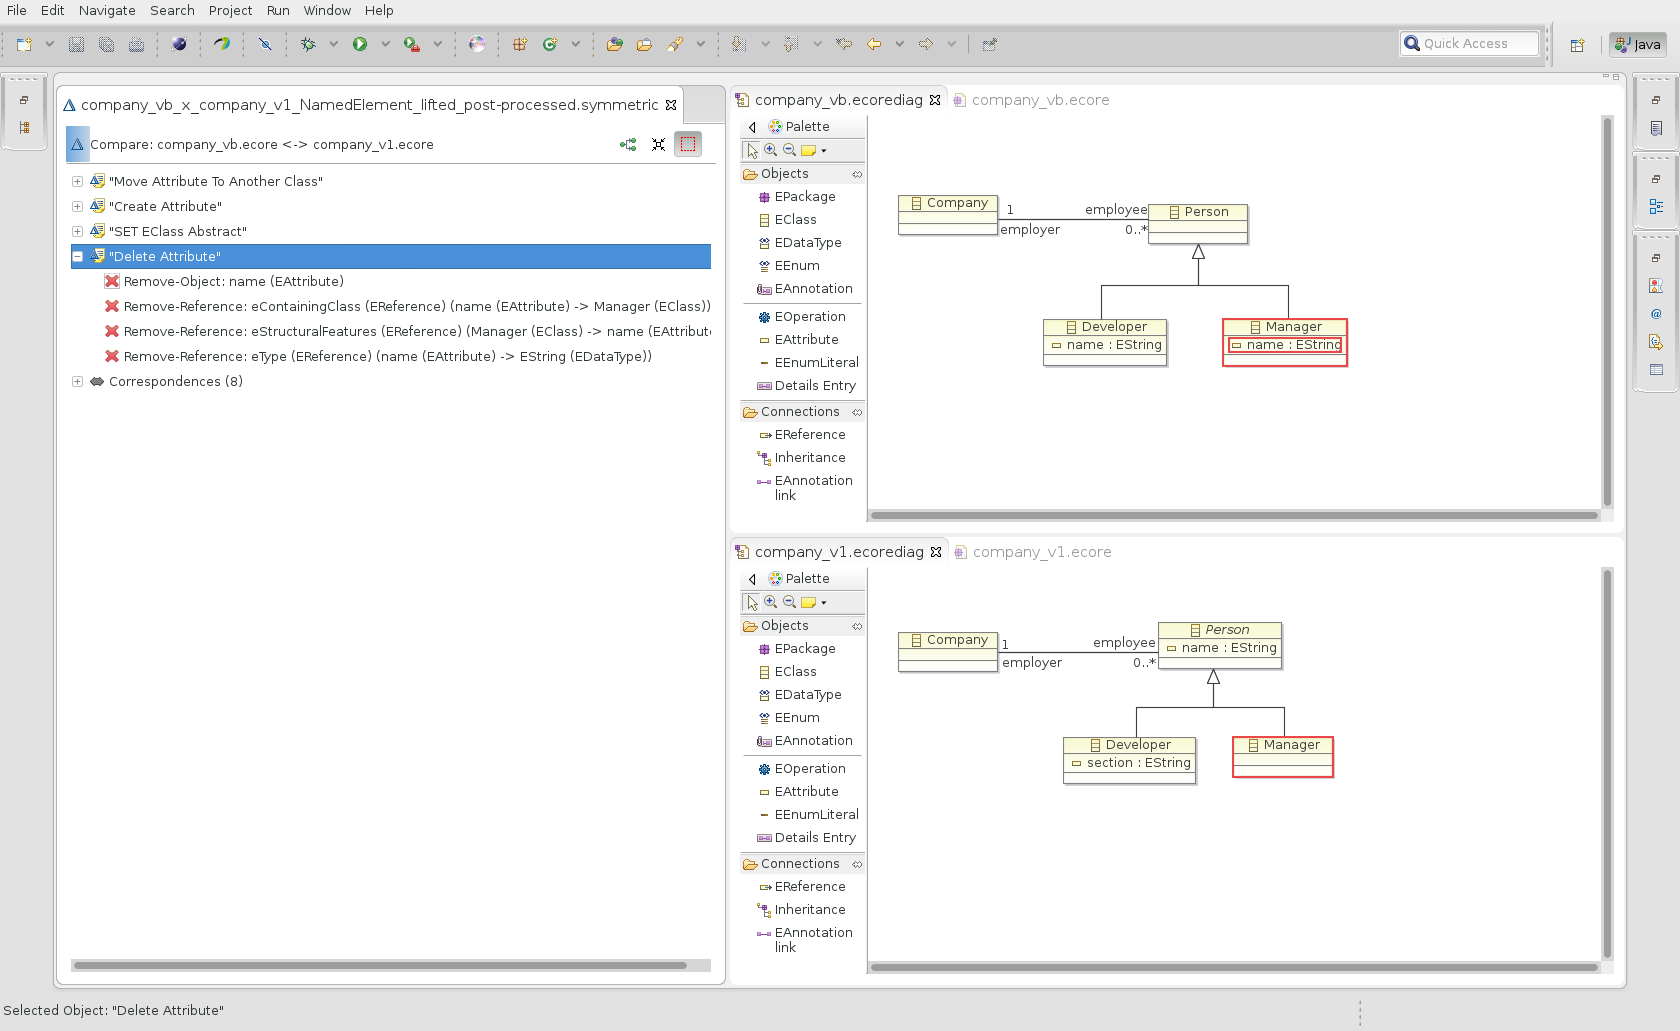
\includegraphics[width=\textwidth]{graphics/silift-tutorial_compare_compare_view.png}
\caption{graphischer Editor (Compare View), atomare Erkennungsregeln}
\label{silift-tutorial_compare_compare_view}
\end{figure}

Wenn wir uns nochmals die oben beschriebenen Änderungen ins Gedächtnis rufen, so lassen sich diesen die Editieroperationen wie folgt zuordnen:

\begin{itemize}
\item \texttt{Move Attribute To Another Class}: Verschiebe Attribut \texttt{name} von \texttt{Developer} nach \texttt{Person}.
\item \texttt{Create Attribute}: Erstelle neues Attribut \texttt{section} in \texttt{Developer}.
\item \texttt{SET EClass Abstract}: Die Klasse \texttt{Person} ist nun \textit{abstrakt}.
\item \texttt{Delete Attribute}: Entferne Attribut \texttt{name} aus \texttt{Manager}.
\end{itemize}

Nochmal zur Erinnerung: Die geliftete Differenz aus Abbildung \ref{silift-tutorial_compare_compare_view} wurde mit Hilfe der atomaren Erkennungsregeln erstellt.
Diese werden wiederum aus den atomaren Editierregeln abgeleitet.
Eine atomare Editierregel kann nicht in noch kleinere Regeln aufgeteilt werden, ohne dass deren Anwendung zu einem inkonsistenten Modell führen würde.
Diese Regeln umfassen i.d.R. das Erstellen (\texttt{create}), Entfernen (\texttt{remove}) und Verschieben (\texttt{move}) von Modellelementen sowie das Ändern von Attributwerten (\texttt{set}).\\
Betrachten wir die beiden Change Sets \texttt{Delete Attribute} und \texttt{Move Attribute To Another Class}.
In diesem Szenario wurde das Attribut \texttt{name} in der Klasse \texttt{Manager} gelöscht und aus der Klasse \texttt{Developer} nach \texttt{Person} verschoben.
Gleichzeitig ließe sich diese Differenz der Modelle jedoch auch als ein \textit{Refactoring} der Vererbungsbeziehung verstehen, indem übereinstimmende Attribute der Unterklassen in die Oberklasse verschoben wurden.
Die für ein solches Refactoring erforderliche Erkennungsregel umfasst also mehrere atomare Regeln.
Um solche Refactorings zu erkennen starten wir SiLift nun zusätzlich mit der komplexen \textit{Rule Base} (vgl. Abb. \ref{silift-tutorial_compare_config_complex}). Die restlichen Einstellungen können Sie aus Abbildung \ref{silift-tutorial_compare_config} übernehmen.

\begin{figure}[H]
\centering
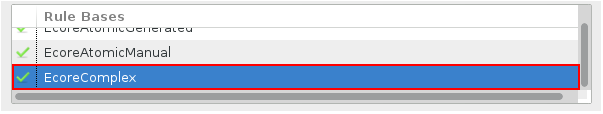
\includegraphics[width=0.5\textwidth]{graphics/silift-tutorial_compare_config_complex.png}
\caption{Einstellungen für das Erstellen einer gelifteten Differenz mit komplexen Erkennungsregeln}
\label{silift-tutorial_compare_config_complex}
\end{figure}

Das Ergebnis ist eine geliftete Differenz die anstatt vier nur noch drei Change Sets beinhaltet  (Abb. \ref{silift-tutorial_compare_compare_view_complex}).
Hier wurden die atomaren Regeln \texttt{Delete Attribute} und \texttt{Move Attribute To Another Class} durch die komplexe Regel \texttt{Pull Up Attribute} ersetzt.

\begin{figure}[H]
\centering
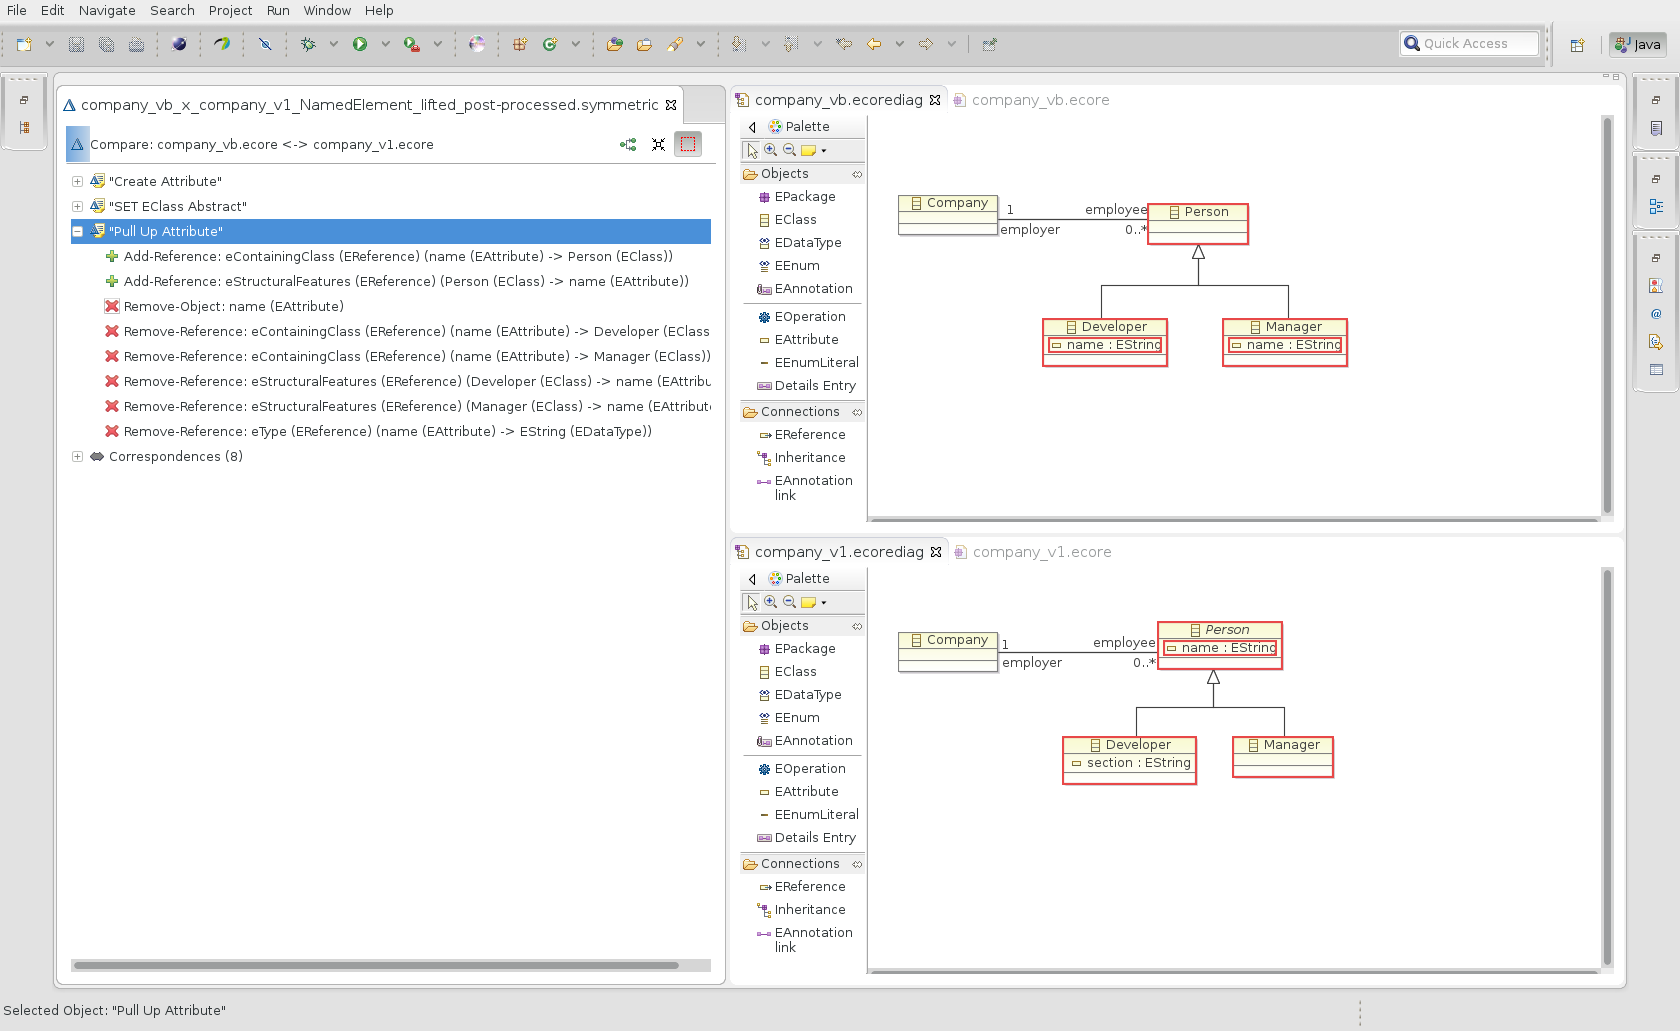
\includegraphics[width=\textwidth]{graphics/silift-tutorial_compare_compare_view_complex.png}
\caption{graphischer Editor (Compare View), komplexe Erkennungsregeln}
\label{silift-tutorial_compare_compare_view_complex}
\end{figure}

Wie bereits erwähnt setzen sich komplexe Regeln aus atomaren und anderen komplexen Regeln zusammen.
Betrachten wir Abbildung \ref{silift-tutorial_compare_atomic_vs_complex}, so deckt die komplexe Regel \texttt{Pull Up Attribute} alle technischen Differenzen der beiden atomaren Regeln \texttt{Delete Attribute} und \texttt{Move Attribute To Another Class} ab.

\begin{figure}[H]
\centering
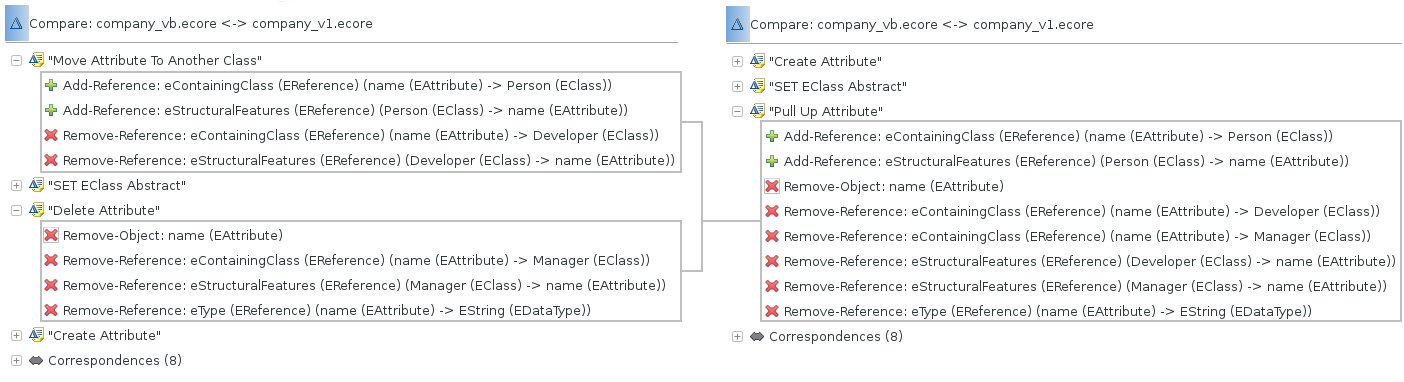
\includegraphics[width=\textwidth]{graphics/silift-tutorial_compare_atomic_vs_complex.png}
\caption{Vergleich atomarer und komplexer Erkennungsregeln}
\label{silift-tutorial_compare_atomic_vs_complex}
\end{figure}

Durch komplexe Erkennungsregeln lassen sich somit größere Refactorings auf eine intuitive Weise darstellen.\\

\newpage

%************************
\subsection{Patchen von Modellen}
%************************
Neben dem semantischen Liften von Differenzen besteht die Möglichkeit einen Patch zu erstellen.\\
Abbildung \ref{silift-tutorial_patching_classdiagrams} zeigt ein typisches Szenario der Patch-Anwendung. 

\begin{figure}[H]
\centering
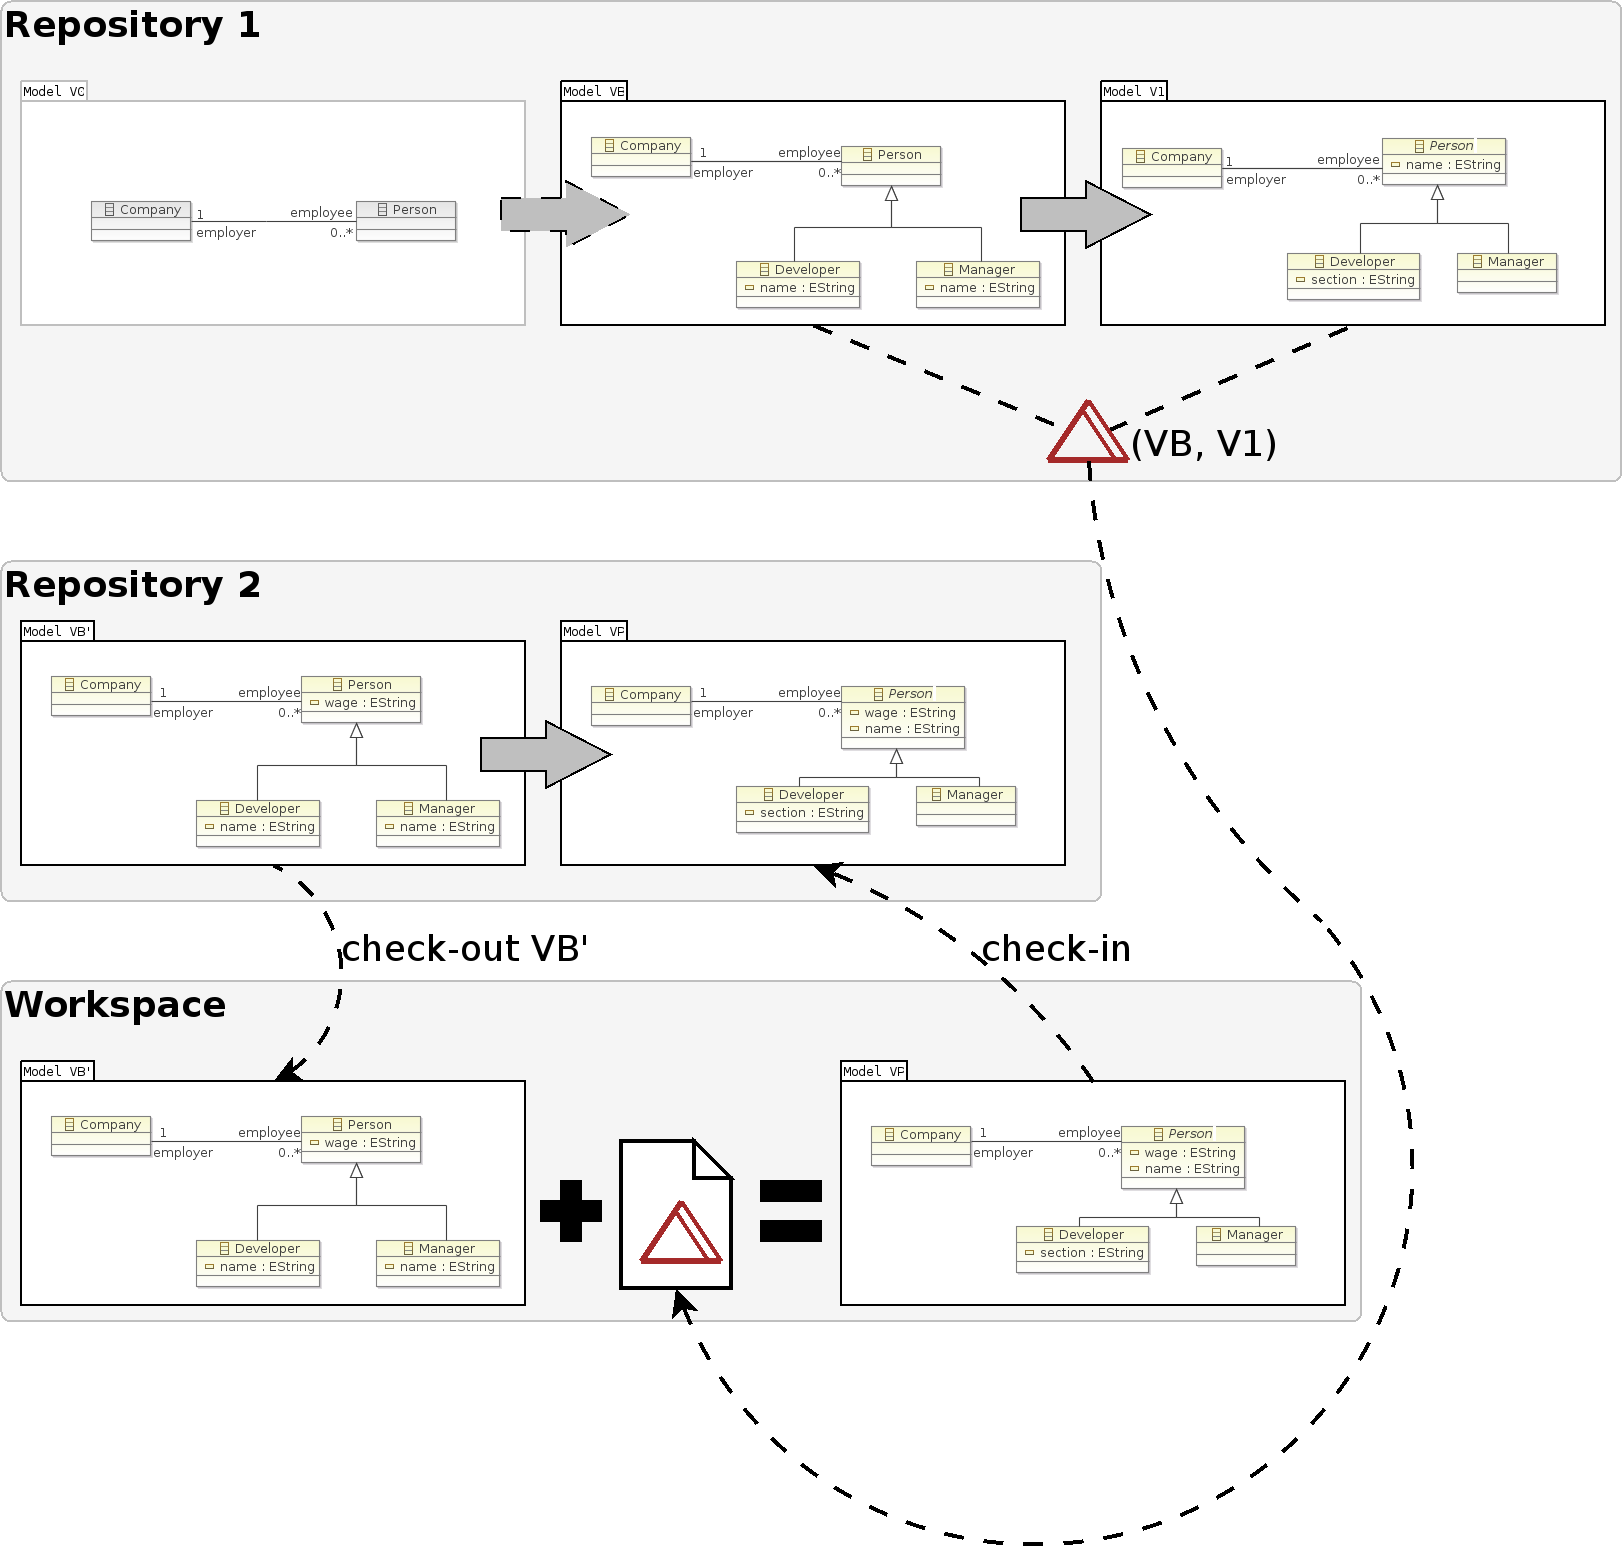
\includegraphics[width=\textwidth]{graphics/silift-tutorial_patching_classdiagrams.png}
\caption{Ablauf einer Patch-Anwendung}
\label{silift-tutorial_patching_classdiagrams}
\end{figure}

\texttt{Repository 1} stellt den Entwichklungsprozess eines Modells dar, welches zu einem bestimmten Zeitpunkt (hier \texttt{Model VB}) in ein zweites Repository übertragen und dort ggf. weiterentwickelt wird (vgl. \ref{silift-tutorial_patching_classdiagrams}, \texttt{Repository 2}, \texttt{Model VB'}). 
Des Weiteren wird das Modell auch in Repository 1 weiterentwickelt bzw. überarbeitet.
Dieses Refactoring soll nun auf Model VB' in Repository 2 angewandt werden, ohne dass die bereist vorgenommenen Änderungen an diesem verloren gehen.
Zu diesem Zweck wird eine asymmetrische Differenz zwischen Model VB und Model V1 gebildet und in Form eines Patches auf Model VB' angewandt (vgl. \ref{silift-tutorial_patching_classdiagrams}, \texttt{Workspace}).\\
Sofern in beiden Modellen Änderungen an dem gleichen Element vorgenommen wurden können Konflikte auftreten. 
An dieser Stelle muss man zwichen der Anwendung eines Patches und dem Mischen von Modellen unterscheiden.
Ein Patch wird i.d.R. auf eine Menge von Kopien eines Modells angewandt.
Sofern diese Kopien parallel weiterentwickelt wurden und dies zu Konflikten führt, werden die betroffenen Änderungen verwofen und durch die des Patches ersetzt.
Bei größeren Änderungen kann es jedoch sein, dass der Patch nicht mehr als Ganzes anwendbar ist. 
Beim Mischen von Modellen wird bei einem Konflikt eine Entscheidung getroffen, welche Änderung beibehalten bzw. verworfen wird (vgl. Abschnitt \ref{sec:merging}).\\

\subsubsection{Erstellen eines Patches}

\begin{figure}[H]
\centering
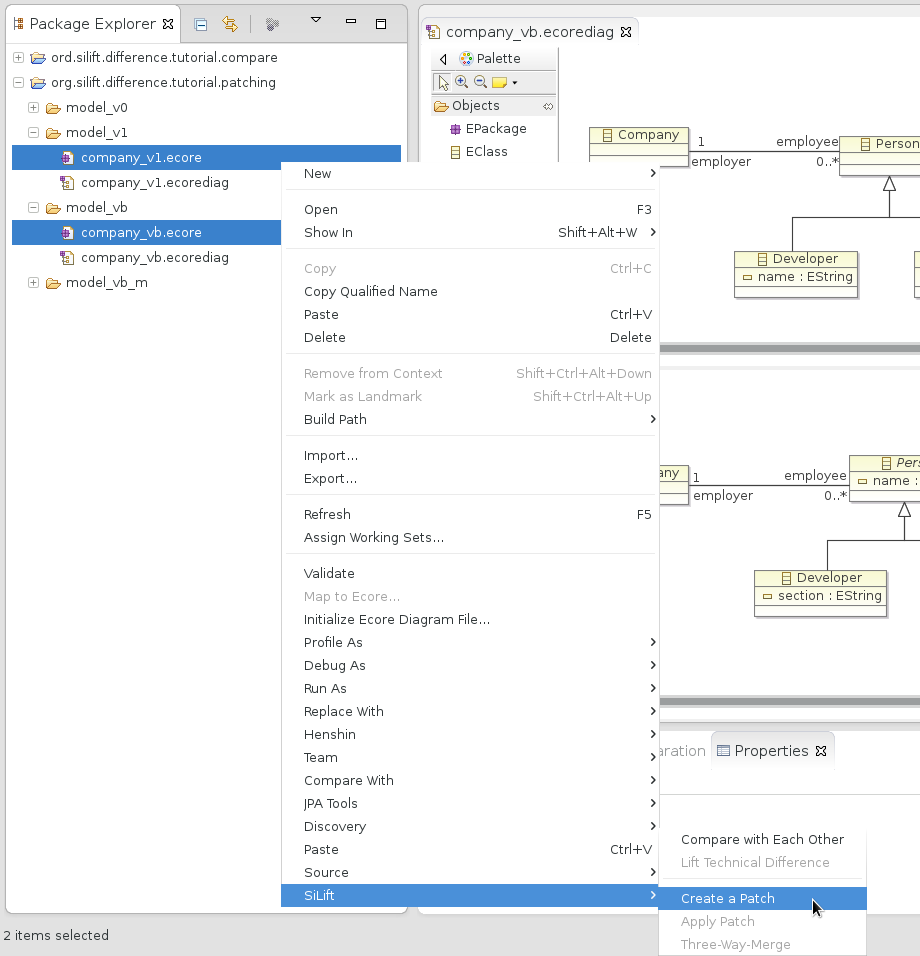
\includegraphics[width=0.8\textwidth]{graphics/silift-tutorial_patching_contextmenu_create.png}
\caption{SiLift: Patch erstellen}
\label{silift-tutorial_patching_contextmenu_create}
\end{figure}


\begin{figure}[H]
\centering
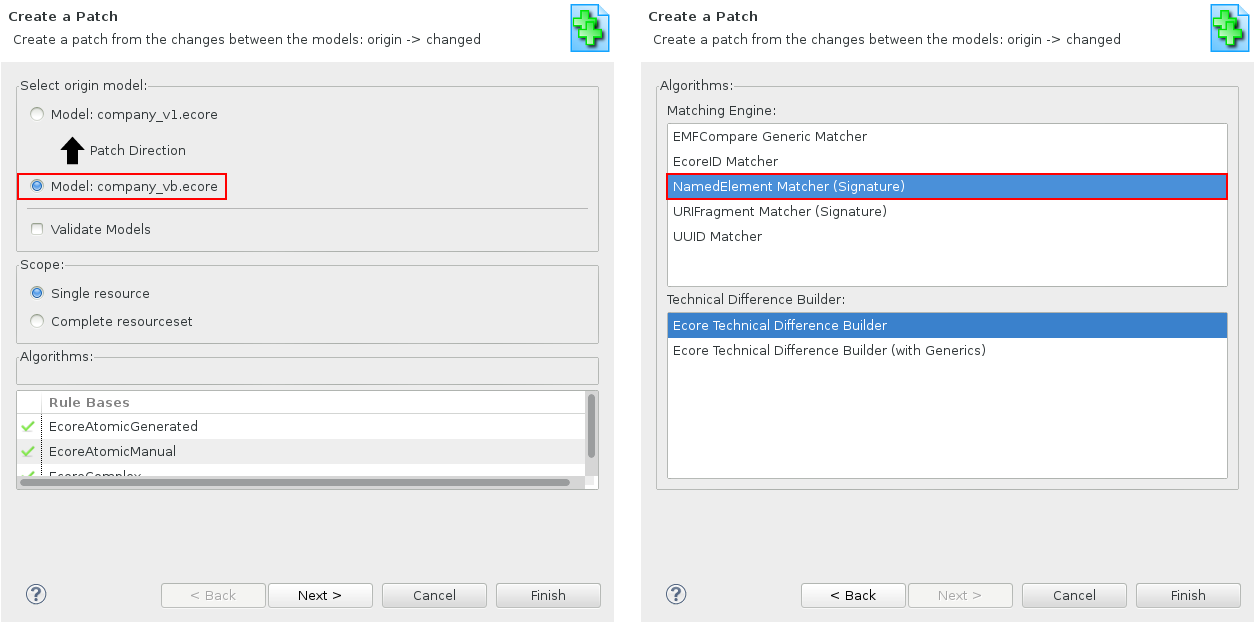
\includegraphics[width=0.8\textwidth]{graphics/silift-tutorial_patching_create_config.png}
\caption{Patch-Config}
\label{silift-tutorial_patching_create_config}
\end{figure}

%************************
\subsection{Mischen von Modellen}
\label{sec:merging}
%************************

\begin{center}
\textbf{ENDE}
\end{center}

\newpage

\section{Links und weitere Informationen}

\begin{itemize}
\item \textbf{SiLift - Benutzerhandbuch für Entwickler}: ...
\item \textbf{EMF-Compare}: \url{http://www.eclipse.org/emf/compare}
\item \textbf{SiDiff}: \url{http://pi.informatik.uni-siegen.de/Projekte/sidiff/}
\item \textbf{SiLift}: \url{http://pi.informatik.uni-siegen.de/Projekte/SiLift/}
\end{itemize} 

%***** Bibliographie  *****
%Die Literatur wird in einem eigenen Dokument im BibTeX Format erfasst: in diesem Fall: referenzen.bib
%\bibliography{referenzen}
% --- Literaturstellen nummerieren
%\bibliographystyle{alphadin}


\end{document}